\chapter{Development}
\section{Considerations}
\subsection{Xcorr}
\subsubsection{Theory}
\subsubsection{Test Matlab}
Before we went any further with the project we investigated which kind of signals which was good to send. We did that by generating a signal, made a delay and then cross-correlated these two signals.
We tried three different signal\\
\textbf{Chirp}:\\
We started with a chirp. We did that because of gut feeling. We thought this would be the best signal to send mostly because it was controlled and not random, and the signal changed characteristic over time.\\

\textbf{Noise}:\\
\textbf{Sinusoid}:\\
\subsection{Output}
UART\\
Sound\\
\section{Convert to BF}
\section{Blackfin}
\textbf{Memory}:\\
\textbf{DMA}:\\
The is a controller circuit on embedded units that can initiate memory read or write cycles. Before the DMA controller can be used we have to initiate it. This is largely platform specific and the way we do it on the blackfin will be described in the algorith implementation chapter. The DMA controller on the blackfin can move data between L1 Cache, Flash or SDRAM and units connected to the DMA Access Bus. The Scope of our project means that we have to use Sport0 (which will be connected to the audio connectors) and internal memory from the L1. 
\textbf{Input}:\\
\textbf{Output}:\\
\textbf{Resources}:\\
Regarding resources on the blackfin we are looking to try to make our own implementation through the project and then compare with the built-in function. We are not trying to do it better but rather get the understanding of what is going on.
We also want to investigate the use of DMA on the blackfin so we do not waste resources on moving data only processing it.
\section{VisualDSP++}
\subsection{Plot}
VisualDSP++ has a built-in function to plot data from the memory of the blackfin. This feature can be used when the blackfin has been flashed and then subsequently halted. To access this feature go into:
\begin{verbatim}
View -> Debug Windows -> Plot -> New
\end{verbatim}
Set name, length and type of the data you want to plot and press \"Add\". This way you can have multiple plots on the same graph. It is also possible to have multiple plots and to save the setting of your plot. An example of plot can be seen on figure~\ref{fig:visualdspplot}.
\begin{figure}[hbpt]
\centering
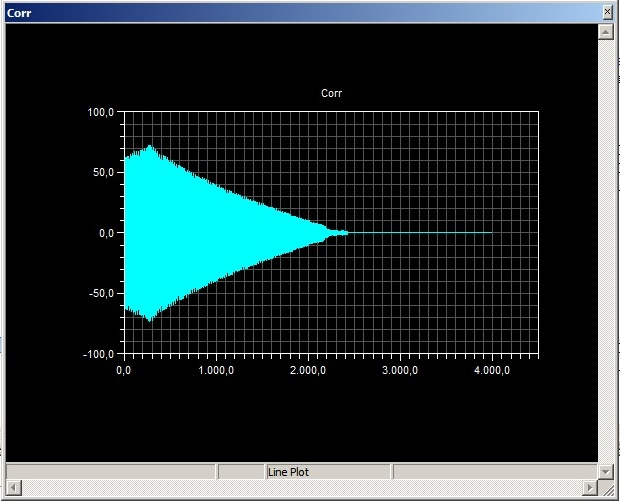
\includegraphics[scale=0.5]{billeder/visualdspplot}
\caption{Plot in VisualDSP++}
\label{fig:visualdspplot}
\end{figure}
\subsection{Memory dump}
A useful feature in VisualDSP++ is Memory dump. We can save the contents of arrays and variables directly onto the computer running VisualDSP++ in ".dat" format. To access this feature go into:
\begin{verbatim}
Memory -> Dump
\end{verbatim}
Set filename, type, size and variable/array name. Matlab can import these files directly.